%!Tex Root=**/main.tex
\subsection{LangSplat}

\begin{Frame}{Key Insight}
	\begin{figure}[htbp]
		\centering
		\begin{annotatedFigureEnv}
			{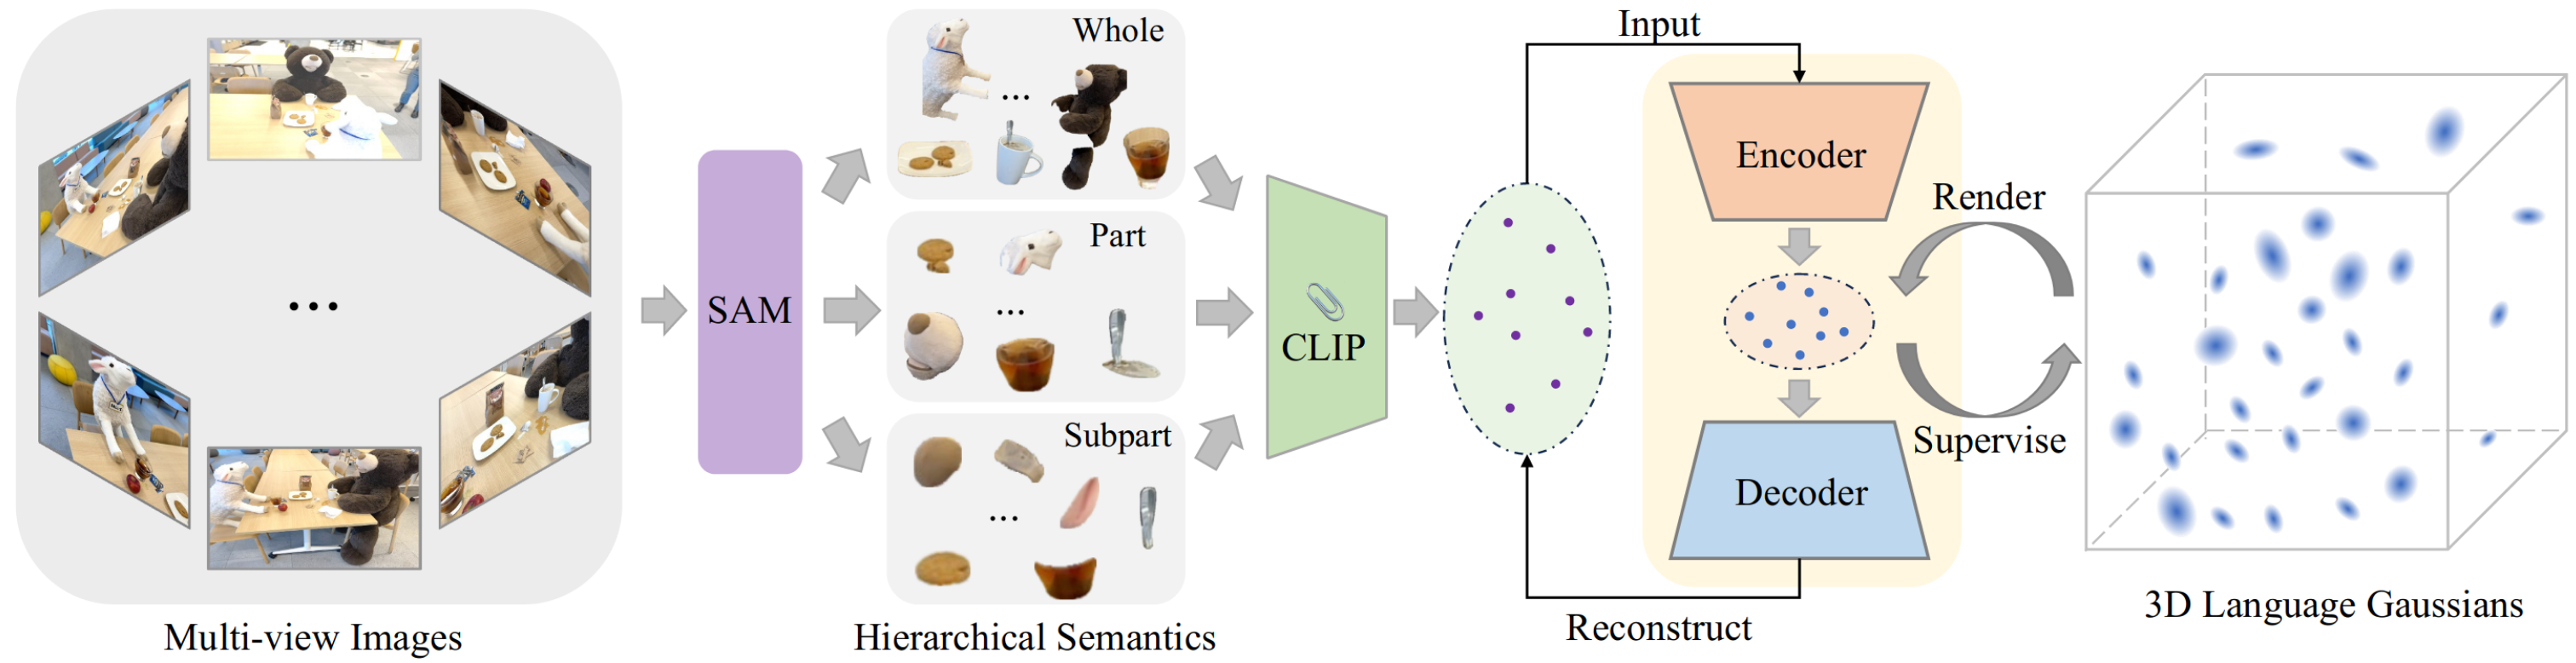
\includegraphics[width=0.8\linewidth]{langsplat-overview.png}}
			\only<2->{\annotatedFigure{0.25,0}{0.55,1}{1}{0.25,0}}
		\end{annotatedFigureEnv}
		\vspace*{0.5ex}
		\caption{Overview of LangSplat}
	\end{figure}
	\vspace*{\fill}
	\begin{enumerate}[<+(1)->]
		\setlength{\itemsep}{1.5ex}
		\item \alert<.(1)>{Accuracy:} SAM outputs to enhance CLIP features.
		      \vspace*{1.5ex}
		      \begin{itemize}
			      \setlength{\itemsep}{1.5ex}
			      \item \alert<.(1)>{CLIP:} image-aligned training leads to ``point-ambiguity''.
			      \item \alert<.(1)>{SAM:} pixel-aligned \& object-centered \& multi-granularity.
		      \end{itemize}
	\end{enumerate}
	\blfootnote{\href{http://arxiv.org/abs/2312.16084}{(CVPR Highlight, 2024) LangSplat: 3D Language Gaussian Splatting}}
\end{Frame}

\begin{Frame}{Key Insight}
	\begin{figure}[htbp]
		\centering
		\begin{annotatedFigureEnv}
			{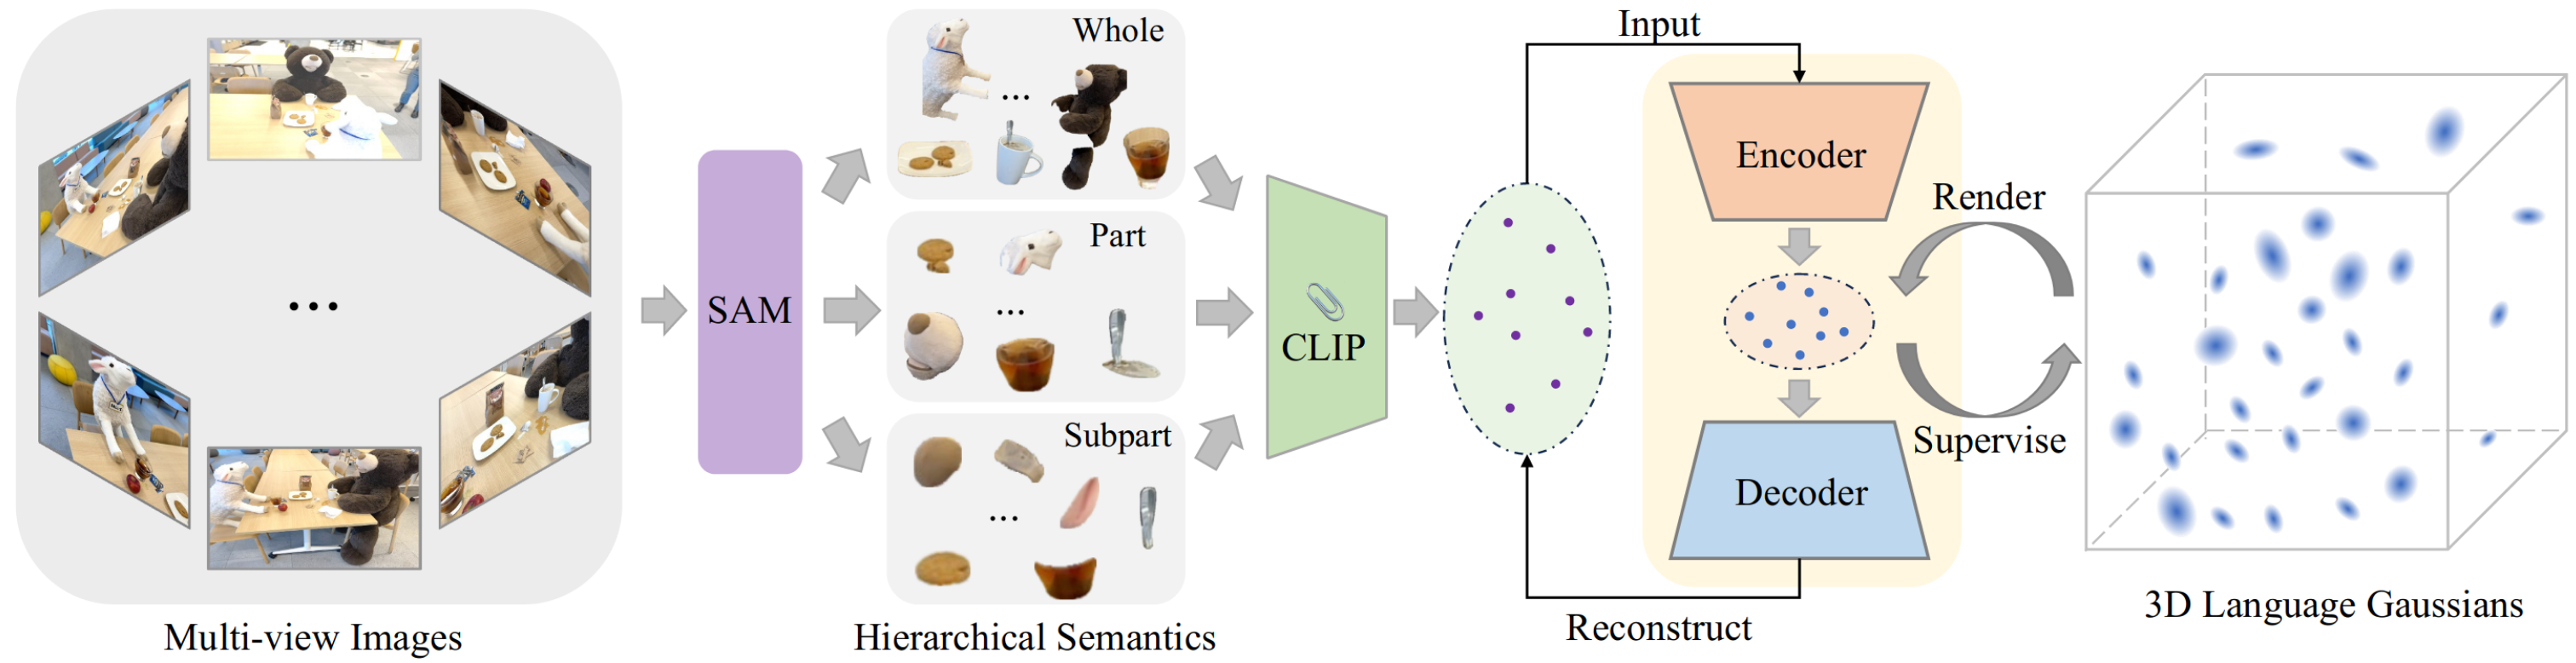
\includegraphics[width=0.8\linewidth]{langsplat-overview.png}}
			\annotatedFigure{0.55,0}{0.82,1}{2}{0.55,0}
		\end{annotatedFigureEnv}
		\vspace*{0.5ex}
		\addtocounter{figure}{-1}
		\caption{Overview of LangSplat}
	\end{figure}
	\vspace*{\fill}
	\begin{enumerate}[<+->]
		\setlength{\itemsep}{1.5ex}
		\setcounter{enumi}{1}
		\item \alert<.>{Efficiency:} an \alert<.>{auto-encoder} to compress latent features.
		      \vspace*{1.5ex}
		      \begin{itemize}
			      \setlength{\itemsep}{1.5ex}
			      \item More complexity and better compression,
			            \vspace*{1.5ex}
			            \par compared with ``speed-up module'' in Feature 3DGS~\autocite{zhouFeature3DGSSupercharging2024apr}.
		      \end{itemize}
	\end{enumerate}
	\blfootnote{In practice, \(\sf \dim = 3\).}
	\blfootnote{\href{http://arxiv.org/abs/2312.16084}{(CVPR Highlight, 2024) LangSplat: 3D Language Gaussian Splatting}}
\end{Frame}

